%% -*- coding: utf-8 -*-
\documentclass[12pt,pagesize,paper=landscape,paper=192mm:108mm]{scrbook} 
%1920x1080 1280x720
\areaset[current]{192mm}{108mm}
\usepackage{calc}
\usepackage[T2A]{fontenc}
\usepackage[utf8]{inputenc}
\usepackage[english,russian]{babel}
\usepackage{microtype}
\usepackage{misccorr}
\usepackage{cmap}
%\usepackage[unicode=true]{hyperref}
\usepackage{graphicx}
\usepackage{amssymb}
\usepackage{amsmath}
%\usepackage{srcltx}
\usepackage{textcomp}
\usepackage{xspace}
%научные символы и смайлики \smiley \frownie
\usepackage{wasysym}
\usepackage{ccicons}
\begin{document}
\begin{titlepage}
  \vspace*{-0.5em}
  \begin{center}    
    \hspace*{3em}
    \begin{minipage}[t]{3em}
      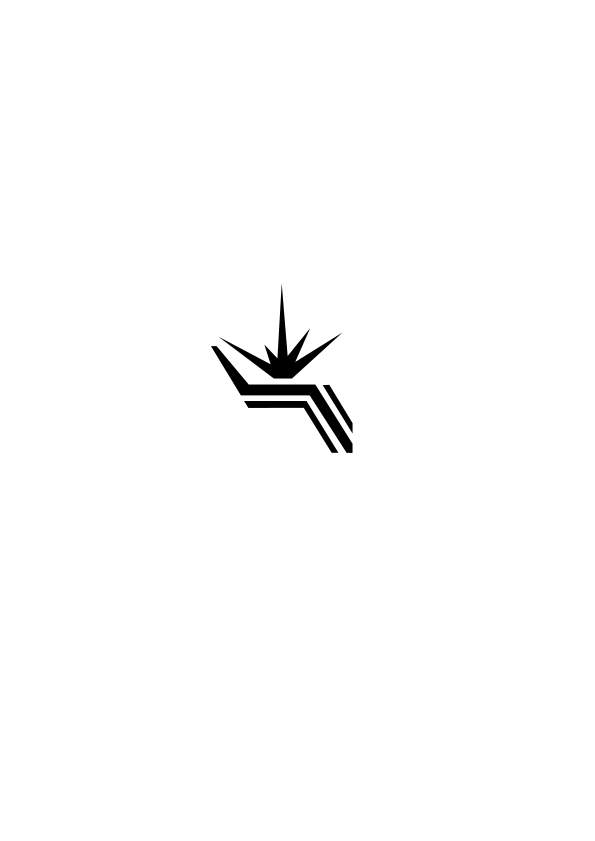
\includegraphics[width=\textwidth]{../BINP-logo}
    \end{minipage}\hfill
    Теоретический отдел ИЯФ им. Г.\,И. Будкера\hfill
    \hspace*{7em}
    \bigskip

    \large
    Пётр Крачков  (ИЯФ СО РАН)
    \bigskip
    \bigskip

    \LARGE Исследование процессов квантовой электродинамики в~сильных
    атомных полях при высоких энергиях
    
    \bigskip

    \normalsize
    (Теоретический семинар 05.05.2016)
    \vfill

    \normalsize
    % \begin{minipage}{0.65\linewidth}
    % \end{minipage}
 %   \vfill

    \normalsize \ccbysa\hspace{0.5em}  Новосибирск 2016
  \end{center}
\end{titlepage}
\end{document}
